\documentclass{article}

\usepackage{times}
\usepackage{geometry}
\geometry{a4paper,left=0.6cm,right=0.7cm,top=2cm,bottom=1cm,columnsep=0.8cm}
\usepackage{fontawesome}
\usepackage[hidelinks]{hyperref}
\usepackage{multicol}
\usepackage{tikz}
\usepackage{hyphsubst}
\usepackage{moresize}
\usepackage{hyphenat}
\usepackage{tabularx}
\usepackage{xcolor}
\usepackage{enumitem}

\newcolumntype{Y}{>{\RaggedRight\arraybackslash}X}

\usepackage{enumitem}
\setlist[itemize]{itemsep=1pt,leftmargin=*,topsep=-10pt}

\definecolor{maincolor}{HTML}{f0fafc}
\definecolor{seccolor}{HTML}{ffffff}
\definecolor{gray}{HTML}{8c94a9}
\definecolor{sidetext}{HTML}{59cee5}

\usepackage[contents={}]{background}
\AddEverypageHook{\begin{tikzpicture}[remember picture,overlay]%
  \node[inner sep=0pt,outer sep=0pt] at (current page.north west) [anchor=north west]{%
  \fcolorbox{maincolor}{maincolor}{%
\begin{minipage}[t][\paperheight][t]{0.3\paperwidth}
        \color{white}
        \hspace{0.08cm}
\end{minipage}}
\fcolorbox{seccolor}{seccolor}{
\begin{minipage}[t][\paperheight][t]{0.67\paperwidth}
        \color{black}
        \hspace{1cm}
\end{minipage}
}
  };%
\end{tikzpicture}
}

\usepackage{enumitem}
\setlist[itemize]{itemsep=-2pt,topsep=0pt,leftmargin=1.08cm}
\renewcommand{\labelitemi}{\textcolor{sidetext}{\footnotesize$\bullet$}}

\setlength{\parindent}{0pt}
\usepackage{paracol}

\begin{document}

\pagestyle{empty}

\columnratio{0.3}
\begin{paracol}{2}
\color{sidetext}
\begin{center}
            \begin{tikzpicture}
            \clip (0,0) circle (1.5cm) node[anchor=center] {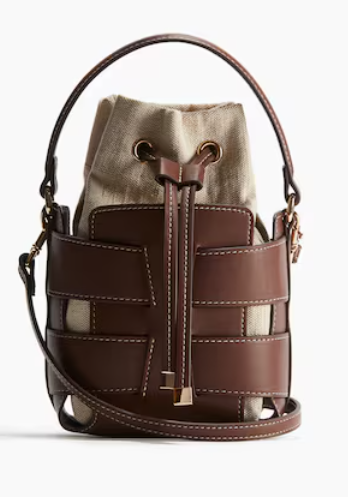
\includegraphics[width=3cm]{8d5f88481fab4014acddf786c5eae388.png}}; 
            \end{tikzpicture}

            ~

         {\color{black}\LARGE \textbf{Pape Saliou Fall}}

         ~

         {\large{Data Scientist}}

        
        \end{center}

{\color{gray}\rule{\linewidth}{0.4pt}} \\

 \begin{tabular}{cl}
            \faPhone{}      & 
            \begin{tabular}{p{0.7\linewidth}}
            {\color{gray}Phone}\\
            {0753481453}
            \end{tabular}
            \\ \\
               \faLinkedin{}      & 
            \begin{tabular}{p{0.7\linewidth}}
            {\color{gray}LinkedIn}\\
            {\href{https://www.linkedin.com/in/pape-saliou-fall-43154a211}{https://www.linkedin.com/in/pape-saliou-fall-43154a211} }
            \end{tabular}
            \\ \\
               \faMapMarker{}      & 
            \begin{tabular}{p{0.7\linewidth}}
            {\color{gray}Address}\\
            {}
            \end{tabular}
            \\ \\
               \faGlobe{}      & 
            \begin{tabular}{p{0.7\linewidth}}
            {\color{gray}Website/Blog}\\
            {\href{}{ }}
            \end{tabular}
            \\
        \end{tabular}
        \vspace{.2cm} \\
        {\color{gray}\rule{\linewidth}{0.4pt}} \\

        {\color{black}{Languages}}

        ~
        
        \begin{tabular}{cl}
            {\Large\faLanguage{}} & \begin{tabular}{l}
             {Français, Anglais} \\
             {\color{gray}Courant}
            \end{tabular} \\
        \end{tabular}
        \vspace{10pt} \\
        {\color{gray}\rule{\linewidth}{0.4pt}} \\

        \vspace{.4cm}

        {\color{black}{Key Skills}}

        ~
        
        \begin{tabular}{ll}
         \begin{minipage}{0.1\linewidth}
         
\includegraphics[width=\linewidth]{picon.png}
         \end{minipage} & {Python} \\[10pt]
         \begin{minipage}{0.1\linewidth}
         
\includegraphics[width=\linewidth]{picon.png}
         \end{minipage} & {Pandas} \\[10pt]
         \begin{minipage}{0.1\linewidth}
         
\includegraphics[width=\linewidth]{picon.png}
         \end{minipage} & {Scikit-learn} \\[10pt]
         \begin{minipage}{0.1\linewidth}
         
\includegraphics[width=\linewidth]{picon.png}
         \end{minipage} & {SQL} \\[10pt]
         \begin{minipage}{0.1\linewidth}
         
\includegraphics[width=\linewidth]{picon.png}
         \end{minipage} & {Data visualisation} \\[10pt]
        \end{tabular}
        
\switchcolumn
\color{black}

\textcolor{black}{\Large \textbf{Professional Summary}} \\

\textcolor{black}{Jeune diplômé en data science spécialisé en analyse de données, modélisation statistique et machine learning. Passionné par la résolution de problèmes complexes et la valorisation de la donnée pour guider la prise de décision. Capable de passer rapidement de l'exploration à la mise en production de solutions prédictives.}\\[8pt]

\textcolor{black}{\Large \textbf{Work Experience}} \\

\colorbox{maincolor}{%
  \begin{minipage}{\linewidth}
    \begin{tabular}{@{}lp{0.72\linewidth}r}
      \begin{minipage}{0.05\linewidth}
        
\includegraphics[width=\linewidth]{picon.png}
      \end{minipage} & 
      {Cursanova} &  
      {\footnotesize {Jun. 2022} {– Mar. 2023} } \\[-10pt]
      & {\color{sidetext}{Stagiaire en Data Science}} & \\
      & {\small {Paris, France}} & \\
    \end{tabular}
\begin{itemize}
    \item Collecte, nettoyage et exploration de jeux de données\\
          Développement de modèles de classification avec scikit-learn\\
          Mise en place de tableaux de bord interactifs (Dash, Plotly)\\
          Présentation des résultats aux équipes métier
\end{itemize}
  \end{minipage}%
}

~ \\[-6pt]

\colorbox{maincolor}{%
  \begin{minipage}{\linewidth}
    \begin{tabular}{@{}lp{0.72\linewidth}r}
      \begin{minipage}{0.05\linewidth}
        
\includegraphics[width=\linewidth]{picon.png}
      \end{minipage} & 
      {} &  
      {\footnotesize {} {} } \\[-10pt]
      & {\color{sidetext}{}} & \\
      & {\small {} } & \\
    \end{tabular}
\begin{itemize}
    \item 
\end{itemize}
  \end{minipage}%
}


\vspace{1cm}

\textcolor{black}{\Large \textbf{Education}} \\


 \begin{tabular}{@{}cp{0.7\linewidth}}
      \begin{minipage}{0.05\linewidth}
        
\includegraphics[width=\linewidth]{picon.png}
      \end{minipage} & \vspace{-12pt}
      {\color{sidetext} {Master 1 Data Science}} \\[-6pt]
      & {Sorbonne Université} \\
      & {} \\
      & {2023} 
    \end{tabular}


~

~

 \begin{tabular}{@{}cp{0.7\linewidth}}
      \begin{minipage}{0.05\linewidth}
        
\includegraphics[width=\linewidth]{picon.png}
      \end{minipage} & \vspace{-12pt}
      {\color{sidetext} {}} \\[-6pt]
      & {} \\
      & {} \\
      & {} 
    \end{tabular}

\vspace{0.5cm}

\textcolor{black}{\Large \textbf{Certifications}} \\

\begin{itemize}[leftmargin=12pt]
\item nk – knp \hfill mai 2023
\item 
\end{itemize}


\end{paracol}



\end{document}